Nous allons présenter dans cette partie les algorithmes utilisés dans cette étude.
\subsection{Parcours de Graham}
Le parcours de Graham est un algorithme publié par Ronald Graham en 1972 pour calculer l'enveloppe convexe d'un ensemble de points dans un espace de dimension 2 et dont la complexité est en $\mathcal{O}(n)$.

Tout d'abord nous effectuons un pré-calcul afin d'alléger le temps d'exécution de l'algorithme par un filtrage de points dit filtrage par pixel dont le principe est le suivant : étant donné des points ayant la même abscisse, 2 de ces points au plus appartiennent à l'enveloppe convexe. Ainsi, il suffit de ne conserver que les points d'ordonnée maximum et minimum pour chaque ensemble de points ayant la même abscisse. Cette opération en $\mathcal{O}(n)$ réduira la taille de l'entrée de manière significative et ne conservera que les points de l'ensemble les plus pertinents pour le parcours de Graham.

\begin{figure}[ht]
\begin{center}
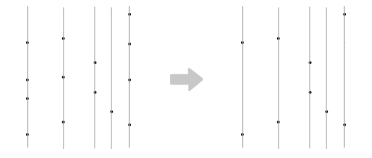
\includegraphics[scale=0.7]{images/tripixel.png}
\caption{Tri pixel}
\end{center}
\end{figure}

Nous allons à présent décrire l'algorithme de Grahamd ont l'idée générale est la suivante : on considère 3 points successifs $P$, $Q$ et $R$ d'abscisse croissant. $Q$ n'appartient à l'enveloppe convexe si et seulement si $R$ est du mauvais côté du demi-plan défini par $PQ$.

\begin{figure}[ht]
\begin{center}
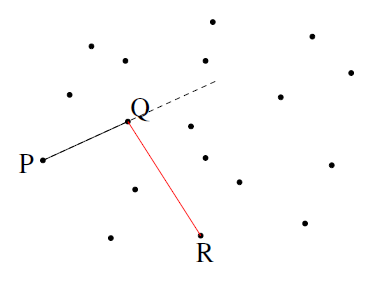
\includegraphics[scale=0.7]{images/graham.png}
\caption{Parcours de Graham}
\end{center}
\end{figure}

On se sert simplement du produit vectoriel afin de déterminer si le triplet \og tourne à droite \fg{} ou \og tourne à gauche \fg{}, on étudie alors le signe du résultat :
\begin{itemize}
\item $0$ : les points sont alignés
\item $>0$ : les points \og tournent à gauche \fg{}
\item $<0$ : les points \og tournent à droite \fg{}
\end{itemize}
En réitérant le processus sur l'ensemble des points on obtient les points constituant l'enveloppe convexe.